\section{Ziele und Grenzen des Softwaretestens}

Die Standarddefinition des Testens nach dem
ANSI/IEEE 1059-Standard besagt, dass Testen der
Prozess der Analyse eines Softwareobjekts ist, um
Unterschiede zwischen bestehenden und erforderlichen
Bedingungen (d.h. Defekte/Fehler/Bugs) zu erkennen
und die Eigenschaften des Softwareobjekts zu bewerten (vgl. \cite{singh2012software}, S.07).
Das Softwaretesten ist daher eine Methode, um zu überprüfen,
ob das Softwareprodukt den erwarteten
Anforderungen entspricht und um sicherzustellen, dass
es frei von Fehlern ist.

Im 21. Jahrhundert ist der Einsatz von Software und
Anwendungen weit verbreitet und kein Bereich bleibt
davon verschont. Die Gesamtmenge der weltweit erstellten,
erfassten, kopierten und verbrauchten Daten ist laut
Statista (vgl. \cite{Statista2021}) bis 2020 rasant auf 64,2
Zettabyte \begin{math}(2^{70})\end{math} angestiegen. Die Nutzer vertrauen ihre sensiblen und privaten Daten
Plattformen an, deren Aufgabe ist es, sie zu schützen. Testen
ist wichtig, weil Softwarefehler teuer oder sogar gefährlich
sein können. Sie können finanzielle
und menschliche Verluste verursachen, und die Geschichte
ist voll von solchen Beispielen:

\noindent
\begin{enumerate}
    \item Im Mai 1996 führte ein Softwarefehler dazu, dass
     den Konten von 823 Kunden einer großen US-Bank 920
     Millionen US-Dollar gutgeschrieben wurden (vgl. \cite{Devi2015}).
    \item Der Airbus A300 der China Airlines stürzte am 26. April
    aufgrund eines Softwarefehlers ab, 1994, bei dem 264 Unschuldige
    ums Leben kamen (vgl. \cite{Takeuch1996}).
\end{enumerate}

Das Testen einer Anwendung hat viele Vorteile. Zu den wichtigsten
gehören die folgenden:


 \textbf{Kosteneffektivität}: Das
rechtzeitige Testen eines IT-Projekts hilft auf
lange Sicht Geld zu sparen. Wenn die Fehler bereits in
der frühen Phase des Softwaretests entdeckt werden,
kostet es weniger, sie zu beheben. Es ist besser, mit
dem Testen früher zu beginnen und es in jeder Phase des
Lebenszyklus der Softwareentwicklung einzuführen.
Regelmäßige Tests sind erforderlich (vgl. \cite{kumar2010software}, S.53), um
sicherzustellen, dass die Anwendung gemäß den Anforderungen entwickelt wird.

\begin{figure}[H]
    \centering
    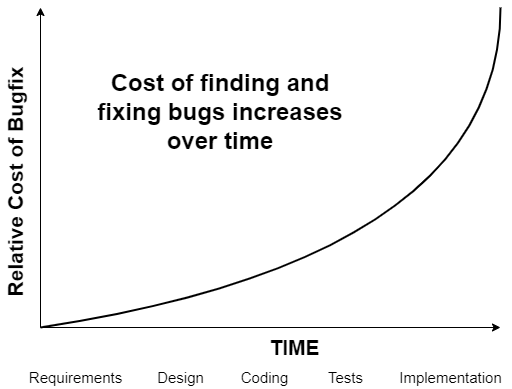
\includegraphics[scale=0.5]{images/Cost-of-fixing-bugs-in-different-phases}
    \caption{Kosten für die Behebung von Fehlern (Bugs) in verschiedenen Phasen (vgl. \cite{kumar2010software})} \label{fig:mof}
\end{figure}


\textbf{Erhöhung der Sicherheit}: Sicherheit ist der anfälligste und
sensibelste Teil des Softwaretestens. Durch Testen wird sichergestellt,
dass die Anwendung über einen minimalen Schutz verfügt. Testen hilft
dabei, Risiken und Probleme früher zu beseitigen. So wird die Anwendung für Nutzer attraktiv,
die vertrauenswürdige Produkte suchen (vgl. \cite{shultz2011software}, S.09).

\textbf{Produktqualität}: Sie ist eine wesentliche
Voraussetzung für jedes Softwareprodukt. Zu den sechs Gruppen von Software-Qualitätsindikatoren
in der ISO-Norm 9126 (vgl. \cite{AlainAbran2010}) gehört die Wartbarkeit, zu der auch die Untergruppe Testbarkeit gehört.
Durch Testen kann die Qualität einer Anwendung sowie ihre Wartbarkeit erhöht werden und so wird dem Kunden sichergestellt,
dass ein Qualitätsprodukt geliefert wird.


Aus diesen Gründen ist das Testen von Software ein
integraler Bestandteil des Softwareentwicklungsprozesses, jedoch hat es Grenzen.
Testen dient nur dazu, das Vorhandensein von potentiellen Fehlern
aufzudecken. Aber es kann nicht sicherstellen, dass
die Software keine Fehler oder Bugs enthält (vgl. \cite{kumar2010software}, S.55).
Dazu können Tests nicht nachweisen, dass ein Produkt unter allen
Bedingungen richtig funktioniert, sondern nur, dass es unter
bestimmten Bedingungen nicht richtig funktioniert (vgl. \cite{kumar2010software}, S.56).



Da das Ziel dieser Arbeit darin besteht, eine \gls{TestSuite} für
eine Webanwendung einzurichten, ist es wichtig zu
definieren, was mit Webanwendung eigentlich gemeint ist.
